The shadow suppression is performed in a fashion similar to what is mention in the paper by Woods \cite{Wood}. The suppression if performed using the Hue- Saturation- Value- (HSV) mapping, The HSV mapping was chosen since it gives very small amounts of false positives and a manageable number of false negatives, while at the same time being fairly simple. We make the assumption that a if a pixel is shadowed the hue remains constant, while there is a decrease in both the value and saturation channels compared to the most likely background at the time.

\begin{figure}[htb]
	\centering
	%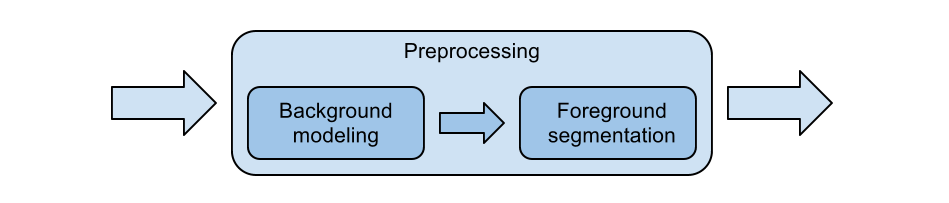
\includegraphics[width=\linewidth]{images/data_flow_preprocessing.png}
	\caption{\textit{Shadow suppression flowchart}}
	\label{fig:shadow_suppression_flow}  %Skapar referens till figuren
\end{figure}

\subsubsection{Implementation}
The Shadow Suppression function is called with a reference to \emph{frame} object containing both a processed version of the probability map, the current frame image as well as the most likely background. The first step is to remap the current frame image and the background model to the HSV-space. The suppression is performed by detecting all contours in the image and, for each contour, go through all the pixels and compare their hue- and saturation values. If a pixel has a the same hue but lower saturation in the image than in the background model is assumed to be caused by a shadow, (eq. 3.19 in Wood \cite{Wood}). All probability map pixels assumed to be shadows are set to zero, and the shadow suppression is thereby finished.